
\section{Approximating solutions of equations}

Which country on Earth has the most people?  If you guess China and India, in that order, you'd be right.  And by a lot compared to other countries.  A very distant third is the United States, with several countries close on our heels.  Here are the population and growth rates estimates from the CIA Factbook from 2011.
\begin{center}
\begin{tabular} {llll}
1. & China & population 1.343 billion & growth rate 0.48\% \\
2. & India & population 1.205 billion & growth rate 1.31\%\\
3. & United States \quad~& population 0.313 billion \quad~  & growth rate 0.90\%\\ 
%4. & Indonesia & population 0.248 billion & growth rate 1.04\% \\
%5. & Brazil & population 0.205 billion & growth rate 1.10\% \\
%6. & Pakistan & population 0.190  billion & growth rate 1.55\% \\
%7. & Nigeria & population 0.170  billion & growth rate 2.55\% \\
%8. & Bangladesh & population 0.161  billion & growth rate 1.58\% \\
% Next are Russia, Japan, and Mexico -- all below .140 billion
\end{tabular}
\end{center}

India's population is growing fastest of these top three, so let's take a closer look.  In the exercises 
% SU check
% Homework/worksheet include asking 
%When will China pass 1.5 billion?
%When will India pass China?
you can explore China and other countries. 
Let's tackle this question: when is India's population projected to pass 1.5 billion?

Start by writing an equation.  The variables are
\begin{center}
\begin{tabular} {l} 
$P=$ population of India (billion people) $\sim$ dep \\
$Y= $ time (years since 2011) $\sim$ indep \\ 
\end{tabular}
\end{center}
Since there is a fixed percentage growth, or at least that's what we're assuming, the population grows exponentially.  The template for an exponential equation is 
$$\text{dep} = \text{start} \ast \text{growth factor} ^ {\text{indep}}$$
For India's population, we know that the growth rate is 
$$r=1.31\% = \frac{1.31}{100} = 1.31 \div 100 = .0131$$
so the corresponding growth factor is 
$$g=1+r=1+.0131=1.0131$$
We also know that the starting population is 1.205 billion in 2011.  We're good to go. The equation is
$$P = 1.205 \ast 1.0131^Y$$

We want to know when India's population will pass 1.5 billion people.  Let's try to figure out the answer by guessing.  Since we're not sure where to start, let's see what the equation projects for 2012, when $Y=1$. 
$$1.205 \ast 1.0131^1 = 1.205 \times 1.0131 \wedge \underline{1} = 1.2208096... \approx 1.221 \text{ billion}$$ 
Hardly budged.  Well, comparatively.  

What about in 5 years?  The corresponding population is 
$$1.205 \ast 1.0131^5 = 1.205 \times 1.0131 \wedge \underline{5} = 1.28614961\approx  1.286\text{ billion}$$ 
Less than 1.5 billion.  Let's try $Y=10$. The equation gives us 
$$1.205 \ast 1.0131^{10} = 1.205 \times 1.0131 \wedge \underline{10} = 1.37276417 \approx 1.373 \text{ billion}$$ 
Still much less than 1.5 billion

This is going slowly.  We would really like to find a point at which the equation gives us more than 1.5 billion. Then we can work backwards from there to narrow things down.  How about 50 years?  
$$1.205 \ast 1.0131^{50} = 1.205 \times 1.0131 \wedge \underline{50} = 2.31223244  \approx 2.312\text{ billion}$$ 
That's too much, but the good news is now we know the answer is between 10 years and 50 years.  

Let's summarize what we have so far in a table.  Notice how we've added a third row to keep track of our progress for our goal.

\begin{center}
\begin{tabular} {|l| |c |c |c |c |c |c |c |c |c |c |c|}\hline
$Y$ & 0 & 1 & 5 & 10 & 50 & \hspace{.25in}~&\hspace{.25in}~&\hspace{.25in}~&\hspace{.25in}~&\hspace{.25in}~&\hspace{.25in}~  \\ \hline
$P$ & 1.205 & 1.221 &1.287  & 1.373 & 2.312 &&&&&&  \\ \hline
vs.\ 1.5 & low & low & low & low & high &&&&&& \\ \hline
\end{tabular}
\end{center}

We know the answer is between 10 and 50 years, and it seems closer to 10, so let's guess 20 years.  In 20 years, the population should be around 1.564 billion.  Where's that 1.564 from?  Just our equation again.  It would be good practice for you to evaluate at $Y=20$ to check.  

The 10 year estimate is too low and the 20 year estimate is too high.  That means the answer is between 10 years and 20 years, so let's split the difference and guess 15 years which gives 1.465 billion.  (Check again, for practice.)  Ooooh, we're getting close.  The population should pass 1.5 billion some time between 15 and 20 years, and likely closer to 15 so let's guess 17 years.  Estimate is  1.504 billion.  Would 16 years have been enough?  That gives 1.484 billion, not quite enough.  Let's add these numbers to our table.

\begin{center}
\begin{tabular} {|l| |c |c |c |c |c |c |c |c  |c|}\hline
$Y$ & 0 & 1 & 5 & 10 & 50 & 20 & 15 & 17& 16 \\ \hline
$P$ & 1.205 & 1.221 &1.287  & 1.373 & 2.312 & 1.564 & 1.465 &1.504  & 1.484  \\ \hline
vs.\ 1.5 & low & low & low & low & high & high & low & high & low \\ \hline
\end{tabular}
\end{center}

According to our equation, the population of the India should pass 1.5 billion after 17 years, which would be in the year 2028.  By the way,  it works to add the year and number. $$2011 + 17 \text{ years } = 2028$$

The strategy we used here is  \textbf{successive approximation}.  That's just a fancy way of saying ``guess-and-check''.  It's called ``successive'' because we're trying to get a closer guess each time.  Typically once we have a value that's too big and one that's too small, we guess a value in between (for example, their average).  This sort of splitting the difference method of guessing is a rough version of the \textbf{bisection method}.  Now you know.

You might be surprised that you're supposed to guess the answer at this point in the course. I mean, in the beginning of the course we didn't have equations, just tables and graphs, and so guessing was all we had to work with.  But now we have actual equations, right?  In previous courses your instructor or textbook might have emphasized getting the ``exact'' answer.  

Here's why it's different in this course.  First, in almost every story in this book the numbers in the problem are approximations, or at least rounded off.  If you start with approximations, no matter how exact your mathematics is, the answers will still be approximate.  Second, even if our numbers started out precisely exact, chances are that the equation is only approximating reality.  Do we really know what the population growth rate will be in India over the next twenty years? And, if the equation is just approximate, then no matter how exact the numbers or the mathematics, the answer will again still be approximate. Last, and this is good news -- we really just want approximations.  Do you really need to know that working out will burn 427.2889 calories?  Isn't 430 calories close enough?

In previous mathematics courses you may have seen ways to solve equations ``exactly,'' and we will talk about those methods in the next chapter of this text.  It is true that successive approximations can taking a long time and, because of that, is a bit annoying.  Solving techniques we'll learn later are much, much quicker.

There are two important reasons for using successive approximations, even if you know quicker solving techniques.   First, the method of successive approximations works in most situations for any type of equation.  Solving methods that we will see later on just work for one type of an equation or another -- one technique for linear equations, a different technique for exponential equations, etc.  That's a lot of different methods to know.  

Second, even if you're going to use a formal equation-solving technique to solve a problem it's a good habit to guess-and-check a bit first to make sure your answer is reasonable.  It is easy to make mistakes when using those formal techniques. There's a rather famous quote here that I like, often falsely attributed to the famous economist John Maynard Keynes, but reportedly from logician Carveth Read in 1898.
\begin{center}
It is better to be vaguely right than exactly wrong.
\end{center}
Something to think about.
% SU -- there is something very similar that appears in MAapproximation.  Check it out.

Okay, enough digression.  Let's check our answer using the graph.
\begin{center}
\scalebox {.8} {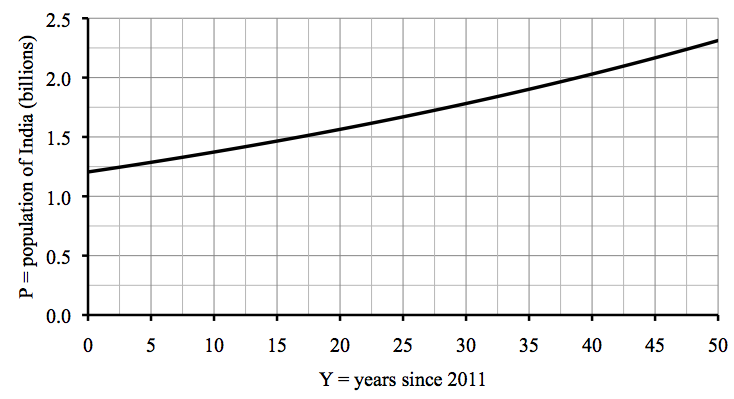
\includegraphics [width=6in] {indiapop.png}}
\end{center}
It looks like 1.5 billion corresponds to just before the unlabeled gridline halfway between 15 and 20.  That line would be 17.5, so the answer of 17 (which was year 2028) looks perfect.

%\newpage

%%\section{Approximating solutions of equations}

 \begin{center}
\line(1,0){300} %\line(1,0){250}
\end{center}

\section*{Homework}

\noindent \textbf{Start by doing Practice exercises \#1-4 in the workbook.}

\bigskip

\noindent \textbf{Do you know \ldots}

\begin{itemize} 
\item What a solution to an equation is? 
\item When you approximate a solution of an equation, as opposed to just evaluating? 
\item How to use successive approximation, including organizing your work in a table? 
\item How to get a reasonable first guess from a graph? 
\item What to do if you do not have a reasonable first guess? 
\item How precise your answer should be? 
\item How to find numbers between given numbers, for example between .3 and .4? 
 \item[~] \textbf{If you're not sure, work the rest of exercises and then return to these questions.  Or, ask your instructor or a classmate for help.} 
\end{itemize}

\subsection*{Exercises}

\begin{enumerate} 
\setcounter{enumi}{4}

\item  The population of China in 2011 was approximately 1.343 billion and growing at around .48\% per year.  An equation estimating the population of China is
$$P = 1.343 \ast 1.0048^Y$$ where $P$ is the population of China (measured in billions) and $Y$ is the years since 2011. \hfill \begin{footnotesize} Source:  CIA Factbook \end{footnotesize}
\begin{enumerate}
\item In what year is China's population projected to reach 1.5 billion?
\item In what year is India's population expected to pass China's?  Remember that we discussed India's population in this section.
 \item Explain how we got the equation for China.
 \item Draw graph showing both equations.
\end{enumerate} 

\item A company who makes electronics was doing great business in 1996, but sales quickly slid after 2000.  Their sales $M$ in millions of \$ $Y$ years from 1996 is given by the following equation $$M = 104.4+11.5Y-1.4Y^2$$
\hfill \emph{Story appears in 3.5 Exercises}
\begin{enumerate}
\item What were the company's sales in 1996, 2000, 2005?
\item The company decided to declare bankruptcy when sales fell below \$20 billion.  In what year was that?  Show how to use successive approximations to estimate the answer to the nearest year. 
\item An analyst had suggested that they close down shop earlier, once sales were below \$50 billion.  In what year did sales fall that low? Again, use successive approximation.
\end{enumerate} 

\item Suppose a special kind of window glass is 1 inch thick and lets through only 75\% of the light. If two thicknesses of this glass are used, the product is 2 inches thick and lets in 56.25\% since $$75\% \text{ of } 75\% = (.75)(.75) = .5625 = 56.25\%$$ 
 \hfill \emph{Story also appears in 3.4 and 5.4 Exercises}
\begin{enumerate}
\item If three thickness of this glass is used, explain why the product is 3 inches think and lets in about 42.19\% of the light.
\item If four thickness of this glass is used, how thick will the product be and what percentage (\%) of the light will be let through?
\item Identify and name the variables, including their units, and write an equation relating them.
\item Use successive approximation to figure out what thickness glass should be used to let through less than 10\% of the light. Display your work in a table.
\item Graph the function.
\end{enumerate} 

\item Wind turbines are used to generate electricity.  For a particular wind turbine, the equation $$W = 2.4 S^3$$ can be used to calculate the amount of electricity generated ($W$ watts) for a given wind speed ($S$ mph), over a fixed period of time.

\hfill \emph{Story also appears in 1.1, 1.3, and 3.3 Exercises}
\begin{enumerate}
\item Make a table showing the amount of electricity produced when the wind speed is 10 mph, 25 mph, and 40 mph. 
\item Draw a graph illustrating this equation.
\item Approximate the wind speed that will generate 12,500 watts of electricity. 
\end{enumerate} 

\item After his first beer, Stephen's blood alcohol content (BAC) was already .04 and as he continued to drink, his BAC level rose 45\% per hour.  The equation is $$S = .04 \ast 1.45^H$$ where $S$ is Stephen's BAC and $H$ is the time, measured in hours.

\hfill \emph{Story also appears in 1.1 \#4 and 3.4 \#1} 
\begin{enumerate}
\item Make a table showing Stephen's BAC at the start of the problem and each of the next four hours.
\item Draw a graph showing how Stephen's BAC changed over time.
\item At a BAC of .10 it is illegal for Stephen to drive.  Approximately when does that happen?
\end{enumerate}  

\item Urban community gardens are catching on.  What was once an abandoned lot down the block is now a thriving 10'$\times$25' vegetable and berry garden for the neighborhood. One neighbor volunteered to donate gravel to make a path around the garden.  The path will be 3 inches deep and the same width all around.   The amount of gravel they need ($G$ cubic feet) is given by the equation  $$G = W^2 + 17.5W$$
where $W$ is the width of the path in feet.  
\begin{center}
\scalebox {.4} {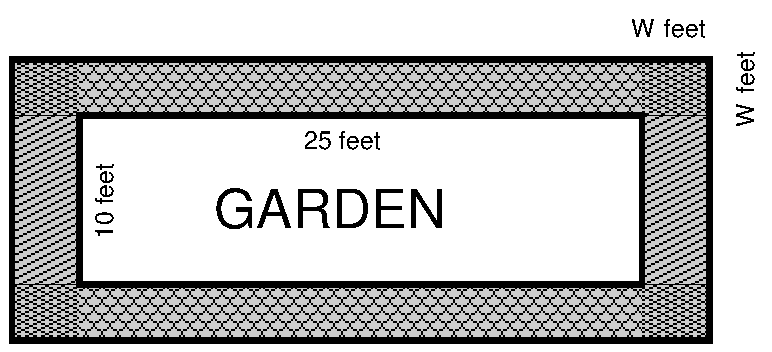
\includegraphics{GravelPath.pdf}}
\end{center}
 \hfill \emph{Story also appears in 2.3 Exercises and 3.5 \#4}
\begin{enumerate}
\item  If the neighbor donates 60 cubic feet of gravel, how wide a path can they build?  Report your answer to two decimal places. 
\item Convert your answer to feet and inches.  Do you think that's a wide enough path? 
\end{enumerate}

\end{enumerate}

